\documentclass[tikz,border=10pt]{standalone}
\begin{document}
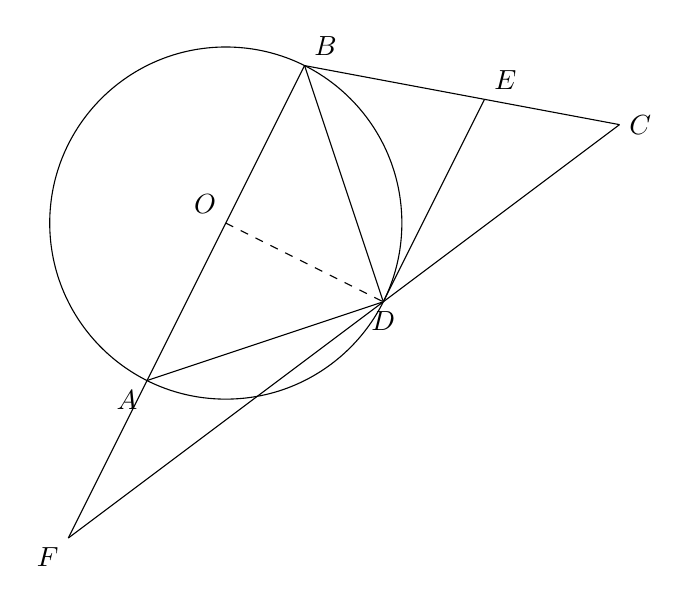
\begin{tikzpicture}
    % Define coordinates based on geometric analysis
    % O is origin
    \coordinate (O) at (0,0);
    % A and B are on the circle, collinear with O. Slope approx 2.
    \coordinate (A) at (-1,-2);
    \coordinate (B) at (1,2);
    % F is on the extension of BA.
    \coordinate (F) at (-2,-4);
    % D is on the circle.
    \coordinate (D) at (2,-1);
    % C is on the extension of FD.
    \coordinate (C) at (5, 1.25);
    % E is on BC. Assuming DE || AB for construction consistency.
    \coordinate (E) at (23/7, 11/7);

    % Draw the circle
    \draw (O) circle ({sqrt(5)});
    
    % Draw lines
    \draw (F) -- (B);       % Line FAB
    \draw (F) -- (C);       % Line FDC
    \draw (B) -- (C);       % Line BEC
    \draw (A) -- (D);       % Chord AD
    \draw (B) -- (D);       % Chord BD
    \draw (D) -- (E);       % Segment DE
    \draw[dashed] (O) -- (D); % Radius OD
    
    % Labels
    \node[below left] at (A) {$A$};
    \node[above right] at (B) {$B$};
    \node[right] at (C) {$C$};
    \node[below] at (D) {$D$};
    \node[above right] at (E) {$E$};
    \node[below left] at (F) {$F$};
    \node[above left] at (O) {$O$};
\end{tikzpicture}
\end{document}
